\documentclass{article}
\usepackage[margin=1in]{geometry}
\usepackage[pdftex]{graphicx}
\usepackage{cite}
\usepackage{color}
\usepackage{listings}
\definecolor{mygreen}{rgb}{0,0.6,0}
\definecolor{mygray}{rgb}{0.9,0.9,0.9}
\definecolor{mymauve}{rgb}{0.58,0,0.52}
\lstset{
  backgroundcolor=\color{mygray},     % choose the background color; you must add \usepackage{color} or \usepackage{xcolor}
  basicstyle=\tiny\ttfamily,  % the size of the fonts that are used for the code
  breakatwhitespace=false,            % sets if automatic breaks should only happen at whitespace
  breaklines=true,                    % sets automatic line breaking
  captionpos=b,                       % sets the caption-position to bottom
  commentstyle=\color{mygreen},       % comment style
  deletekeywords={...},               % if you want to delete keywords from the given language
  escapeinside={\%*}{*)},             % if you want to add LaTeX within your code
  extendedchars=true,                 % lets you use non-ASCII characters; for 8-bits encodings only, does not work with UTF-8
  frame=single,                       % adds a frame around the code
  keepspaces=true,                    % keeps spaces in text, useful for keeping indentation of code (possibly needs columns=flexible)
  keywordstyle=\color{blue},          % keyword style
  language=Verilog,                   % the language of the code
  morekeywords={*,...},               % if you want to add more keywords to the set
  numbers=left,                       % where to put the line-numbers; possible values are (none, left, right)
  numbersep=5pt,                      % how far the line-numbers are from the code
  numberstyle=\tiny\color{mygray},    % the style that is used for the line-numbers
  rulecolor=\color{black},            % if not set, the frame-color may be changed on line-breaks within not-black text (e.g. comments (green here))
  showspaces=false,                   % show spaces everywhere adding particular underscores; it overrides 'showstringspaces'
  showstringspaces=false,             % underline spaces within strings only
  showtabs=false,                     % show tabs within strings adding particular underscores
  stepnumber=2,                       % the step between two line-numbers. If it's 1, each line will be numbered
  stringstyle=\color{mymauve},        % string literal style
  tabsize=1,                          % sets default tabsize to 2 spaces
  %title=\lstname                      % show the filename of files included with \lstinputlisting; also try caption instead of title
}
\title{EEE 178: Homework 1}
\date{\today}
\author{Curtis Muntz}


\begin{document}
\maketitle
Note: MATLAB code is attached at the end of this document.
\begin{enumerate}
  \item Read Image
    \begin{itemize}
      \item See matlab code (attached)
    \end{itemize}
  \item Display Image
    \begin{itemize}
       \item See matlab code (attached)
    \end{itemize}

  \item Transform the color to gray level
    \begin{itemize}
    \item See matlab figure (attached)
    \end{itemize}

  \item Display Histogram of the image
    \begin{itemize}
      \item See matlab code and figure (attached)
    \end{itemize}
  \item Resize the image to 200x200 pixels
    \begin{itemize}
      \item See matlab code and figure (attached)
    \end{itemize}

  \item Transform the image to binary using two different threshold values
    \begin{itemize}
      \item See matlab code and figures (attached) Standard threshold of 0.5 was used and the second binary image used a 0.1 threshold
    \end{itemize}

  \item How many bytes are needed to represent a color image of 200 by 200 pixels with 16 levels of gray?
  \begin{itemize}
    \item $200*200 = 40000$
    \item $16=2^x$
    \item $x = 4$
    \item $1$ byte = $8$ bits
    \item $40000$ $*$ $4$ $*$ $\frac{1}{2}$ = $80000$ bytes or $8KB$ (uncompressed)
  \end{itemize}

  \item Do you think that image difference provides a good tool for image comparison? explain.
  \begin{itemize}
    \item It depends on the two images. If the two images are visibly different, subtracting them from one anoter doesn't necessarily tell us a lot visually; for example taking an image and subtracting a very dark image will produce nearly the same first image. It can help show things like error after an image is quantized. This error has uses in other applicaitons such as predictive compression algorithms.
  \end{itemize}

  \item Perform addition and subtraction of two images.
  \begin{itemize}
    \item See matlab code and figures (attached)
  \end{itemize}

  \item Discuss some of the advantages and applications of binary images.
  \begin{itemize}
    \item Binary images are important because they can be used to encode data for a computer to read. Such encoders can be seen in barcodes, QR codes, fingerprints, etc. Binary images are easily compressible, and even uncompressed consume very little data as they only store 1 bit per pixel.
  \end{itemize}
\end{enumerate}

% %figures
%       \begin{figure}[ht!]
%         \centering
%         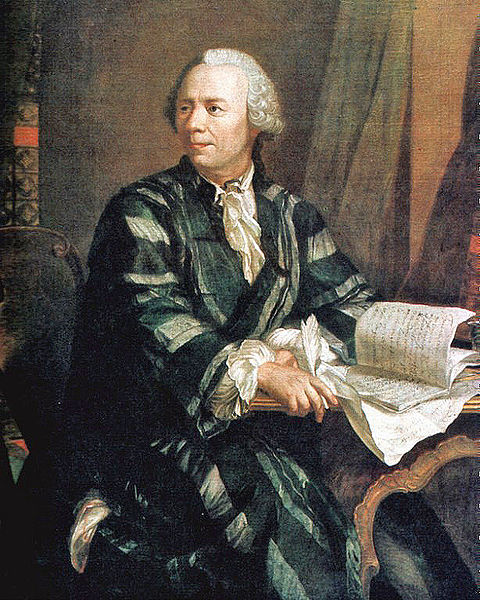
\includegraphics[width=90mm]{./imgs/originalimg.png}
%         \caption{Original Image}
%         \label{original}
%       \end{figure}

%       \begin{figure}[ht!]
%       \centering
%       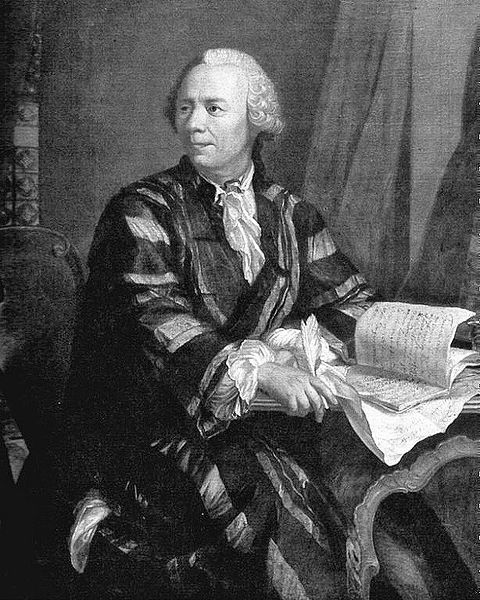
\includegraphics[width=90mm]{./imgs/grayimg.png}
%       \caption{Gray Image}
%       \label{gray}
%       \end{figure}

%       \begin{figure}[ht!]
%       \centering
%       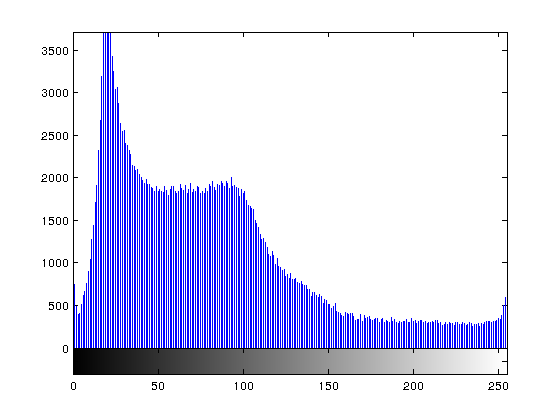
\includegraphics[width=90mm]{./imgs/histogram.png}
%       \caption{Histogram of Figure \ref{gray}}
%       \label{histogram}
%       \end{figure}

%      \begin{figure}[ht!]
%       \centering
%       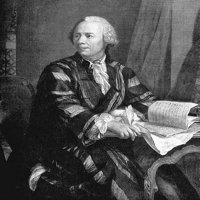
\includegraphics{./imgs/resized.png}
%       \caption{Resized Image}
%       \label{resized}
%       \end{figure}

%     \begin{figure}[ht!]
%     \centering
%     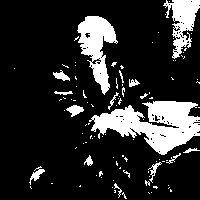
\includegraphics[width=90mm]{./imgs/binary1.png}
%     \caption{Binary using standard threshold}
%     \label{binary1}
%     \end{figure}

%     \begin{figure}[ht!]
%     \centering
%     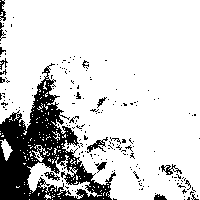
\includegraphics[width=90mm]{./imgs/binary_nonstandard.png}
%     \caption{Binary using 0.1 threshold}
%     \label{binary2}
%     \end{figure}

 
%     \begin{figure}[ht!]
%     \centering
%     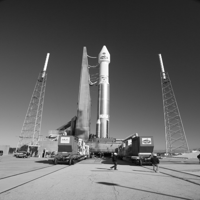
\includegraphics[width=90mm]{./imgs/rocket1.png}
%     \caption{Rocket 1}
%     \label{rocket1}
%     \end{figure}

%     \begin{figure}[ht!]
%     \centering
%     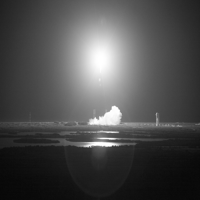
\includegraphics[width=90mm]{./imgs/rocket2.png}
%     \caption{Rocket 2}
%     \label{rocket2}
%     \end{figure}

%     \begin{figure}[ht!]
%     \centering
%     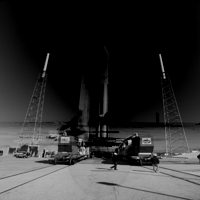
\includegraphics[width=90mm]{./imgs/difference.png}
%     \caption{Difference between Rocket 1 and Rocket 2}
%     \label{difference}
%     \end{figure}

%     \begin{figure}[ht!]
%     \centering
%     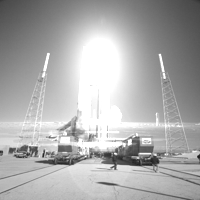
\includegraphics[width=90mm]{./imgs/sum.png}
%     \caption{Sum of Rocket 1 and Rocket 2}
%     \label{sum}
%     \end{figure}
% \vfill\eject
% \eject

% \begin{lstlisting}[language=C++]{Name=MATLAB}
%   %EEE178 HW1
%   clear all;
%   close all;
%   clc;
%   clf;
%   cd imgs
%   %file paths
%   eulerimg = '/home/me/Pictures/480px-Leonhard_Euler_2.jpg';
%   rocket1 = '/home/me/Pictures/2014-1150.jpg';
%   rocket2 = '/home/me/Pictures/2014-1211.jpg';

%   %--------%
%   % part 1 %
%   %--------%
%   %load euler image into a matrix
%   [I,map] = imread(eulerimg,'jpg');
%   imfinfo(eulerimg);

%   %--------%
%   % part 2 %
%   %--------%
%   %display image
%   imshow(I);
%   imwrite(I,'originalimg.png');
%   %--------%
%   % part 3 %
%   %--------%
%   %transform image to gray level
%   figure('name', 'Gray Image');
%   grayI = rgb2gray(I);
%   imshow(grayI);
%   imwrite(grayI,'grayimg.png');

%   %--------%
%   % part 4 %
%   %--------%
%   %display image histogram
%   figure('name', 'Histogram');
%   imhist(grayI);
%   print -dpng histogram_bad;

%   %--------%
%   % part 5 %
%   %--------%
%   %resize image to 200x200 pixels
%   figure('name', 'Resized to 200x200');
%   resized = imresize(grayI, [200,200]);
%   imshow(resized);
%   imwrite(resized, 'resized.png');

%   %--------%
%   % part 6 %
%   %--------%
%   %transform image to binary, use two different thresholds to compare
%   %using standard threshold
%   figure('name', 'Binary Image');
%   binary1 = im2bw(I);
%   imshow(binary1);
%   imwrite(binary1, 'binary1.png');
%   %using non-standard threshold
%   figure('name', 'Binary with non-standard threshold value');
%   binary2 = im2bw(I,0.2);
%   imshow(binary2);
%   imwrite(binary2, 'binary_nonstandard.png');

%   %--------%
%   % part 9 %
%   %--------%
%   % %diffing using the binary images from before:
%   %loading color rocket images into matrices
%   [J,map]=imread(rocket1, 'jpg');
%   [K,map]=imread(rocket2, 'jpg');
%   %resizing them so i can add/subtract them from each other
%   Jsized = imresize(J, [1024,768]);
%   Ksized = imresize(K, [1024,768]);
%   %grayscaling
%   Jgray=rgb2gray(Jsized);
%   Kgray = rgb2gray(Ksized);
%   %differencing
%   figure('name', 'Rocket1');
%   imshow(Jgray);
%   imwrite(Jgray, 'rocket1.png');
%   figure('name', 'Rocket2');
%   imshow(Kgray);
%   imwrite(Kgray, 'rocket2.png')

%   figure('name','Difference between rockets');
%   diff1=Jgray-Kgray;
%   imshow(diff1);
%   imwrite(diff1, 'difference.png');
%   %summing
%   figure('name', 'Sum of two rockets');
%   sum1=Jgray+Kgray;
%   imshow(sum1);
%   imwrite(sum1, 'sum.png');
%   cd ..
% \end{lstlisting}
\end{document}